%%%%%%%
% Ch2 %
%%%%%%%

\chapter{Redresseur à diodes}
	
	Ils sont simples, bon marché et ne nécessitent aucun réglage, délivrent une tension continue essentiellement constante sur base d'une tension alternative. Il existe deux catégories de charges à alimenter, celles pour lesquelles il faut délivrer une tension continue lisse et celle pour lesquelles il faut limiter la déformation du signal. Les équipements électroniques appartiennent à la 1re catégorie, c'est pourquoi on retrouve un condensateur connecté entre les bornes de sortie qui permet de lisser le signal redressé. Les machines à courant continu, charges dites $RLE$, appartiennent à la 2e catégorie, nécessite un redresseur à thyristors (\textbf{commandable}) puisque celui à diode est \textbf{non-commandable}. La liste des symboles utilisés est reprise ci-dessous.
	
	\begin{center}
	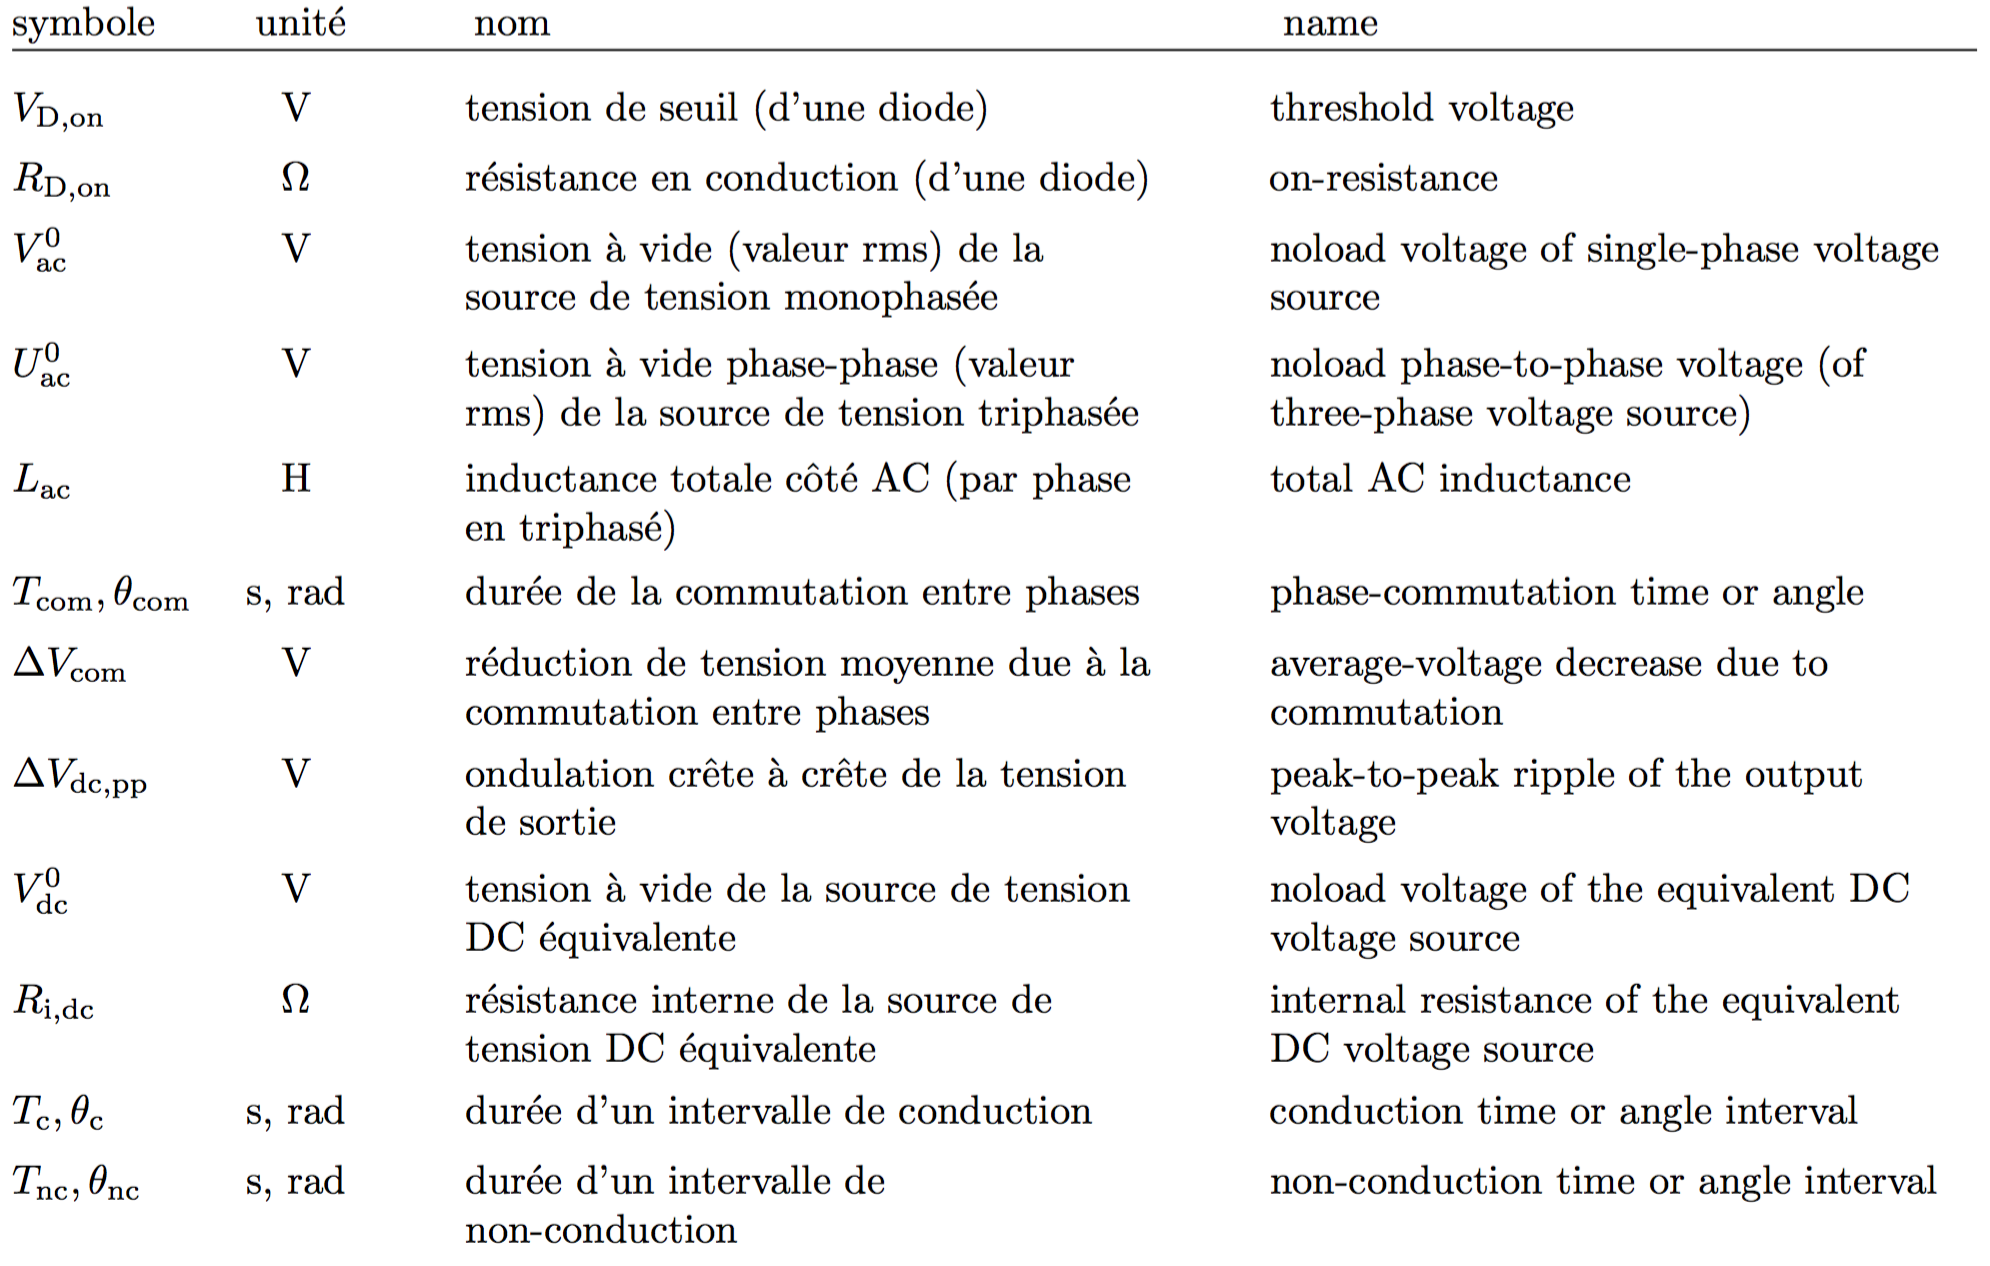
\includegraphics[scale=0.45]{ch2/1}
	\captionof{table}{Liste des symboles.}
	\end{center}
	\newpage
	
	\section{Caractéristique des diodes}
		La figure ci-dessous reprend la représentation réelle à idéalisée de la diode. Elle est \textbf{conductrice} ou passante pour $v_D=v_{AK}$ positive. La tension dépend alors peu du courant $i_D$. 
		
		\begin{center}
		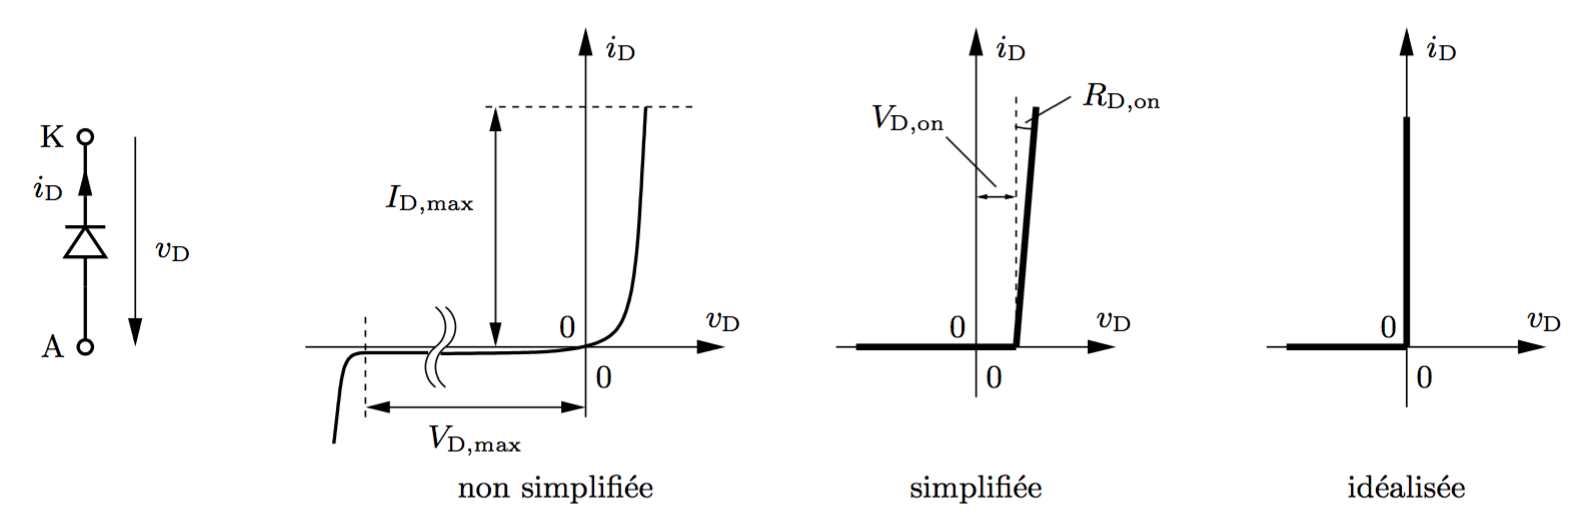
\includegraphics[scale=0.45]{ch2/2}
		\captionof{figure}{}
		\end{center}			
		
		Le courant maximum qu'elle peut supporter, noté $i_{D,max}$ dépend de sa construction, sa taille et du radiateur, refroidisseur sur lequel elle est montée et peut atteindre plusieurs $kA$ pour celles sur le commerce. Pour les diodes de puissance, le transfert de chaleur vers le radiateur est essentiel. De plus elles ont une faible \textbf{inertie thermique} vu leur taille. Pour le modèle simplifié, on a en conduction :
		\begin{equation}
			v_D = v_{D,on} + R_{D,on} i_D
		\end{equation}
		où $v_{D,on}$ est appelé \textbf{tension de seuil} et est de l'ordre du volt. Sauf pour les basses tensions (dizaine de volts ou moins), on négligera cette tension $v_D$, car elle influence peu les caractéristiques macroscopiques des convertisseurs. On n'oubliera cependant pas qu'il existe une \textbf{perte de conduction} instantanée $P_D(t) = v_D(t)i_D(t)$. \\
	
		Pour ce qui est de l'état \textbf{bloquant} ou \textbf{bloqué}, il se manifeste lorsque $v_D < 0$ et $i_D$ sera négatif, mais négligeable. La tension inverse maximum qu'on peut appliquer est notée $v_{D,max}$ et vaut plusieurs $kV$. Les diodes de puissance sont utilisées à de faibles \textbf{fréquences de commutation} (50 ou 60 $Hz$).
	
	\section{Charge inductive générique et circuits redresseurs élémentaires à une ou deux diodes}
		\subsection{Charge RLE générique}
			Pour l'étude des circuits, on considérera une charge inductive générique RLE. Ces paramètres sont supposés constants c'est-à-dire que leur variation sur un cycle d'alimentation AC est négligeable. Ceci représente par exemple le circuit d'induit d'une MCC ($E_{dc}\neq 0$) ou son circuit d'excitation ($E_{dc}=0$). L'équation différentielle pour la tension aux bornes de la charge est :
			\begin{equation}
				v_{dc} = E_{dc} + R_{dc}i_{dc} + L_{dc}\frac{di_{dc}}{dt}.
			\end{equation}
			En régime établi et en introduisant la \textbf{tension moyenne} $V_{dc}$ et le \textbf{courant moyen} $I_{dc}$, on a :
			
			\begin{equation}
				V_{dc} = E_{dc} + R_{dc} I_{dc}.
			\end{equation}
			La charge étant alimenté par un redresseur à diode, $i_{dc}$ et $I_{dc}$ ne peuvent pas être négatifs et si $E_{dc}$ est trop élevé, le courant est nul. On a :
			\begin{equation}
				I_{dc} = max\left(\frac{V_{dc} - E_{dc}}{R_{dc}}, 0\right).
			\end{equation}
			
			L'inductance de la charge tend à lisser le courant. C'est d'autant plus le cas que la constante de temps $\tau = L_{dc}/R_{dc}$ est grande par rapport à $T=1/f$ du réseau. Pour les ponts monophasé ou triphasé, c'est l'intervalle de temps $T/2$ ou $T/6$ qui importe. Dans le cas d'une MCC, les ondulations de la tension impliquent une ondulation du courant et donc une ondulation du \textbf{couple électromagnétique}, ce qui est dérangeant. On peut donc adjoindre une inductance extérieure si c'est insuffisant, au détriment de performances dynamiques réduites en cas de commande de couple, vitesse ou de position de l'entraînement électrique. 
			
		\subsection{Circuits redresseurs élémentaires avec une diode et une charge R, ER ou EL}
			\subsubsection{Avec charge R}
				La figure ci-dessous représente un circuit avec une source de tension AC de fréquence $f$ idéale raccordée à une diode idéale et une résistance avec $R_{dc}$ constante. Dans ce cas, $i_{ac}(t)=i_{dc}(t)$ à tout instant. La diode n'est passante que lorsque $v_{ac}(t)>0$, avec $v_{dc}(t)=v_{ac}(t)$ et $i_{dc}=v_{ac}(t)/R_{dc}$. La diode est bloquante lorsque $v_D=v_{ac}<0$, avec $v_{dc}=0=i_{dc}$.
				
				\begin{center}
					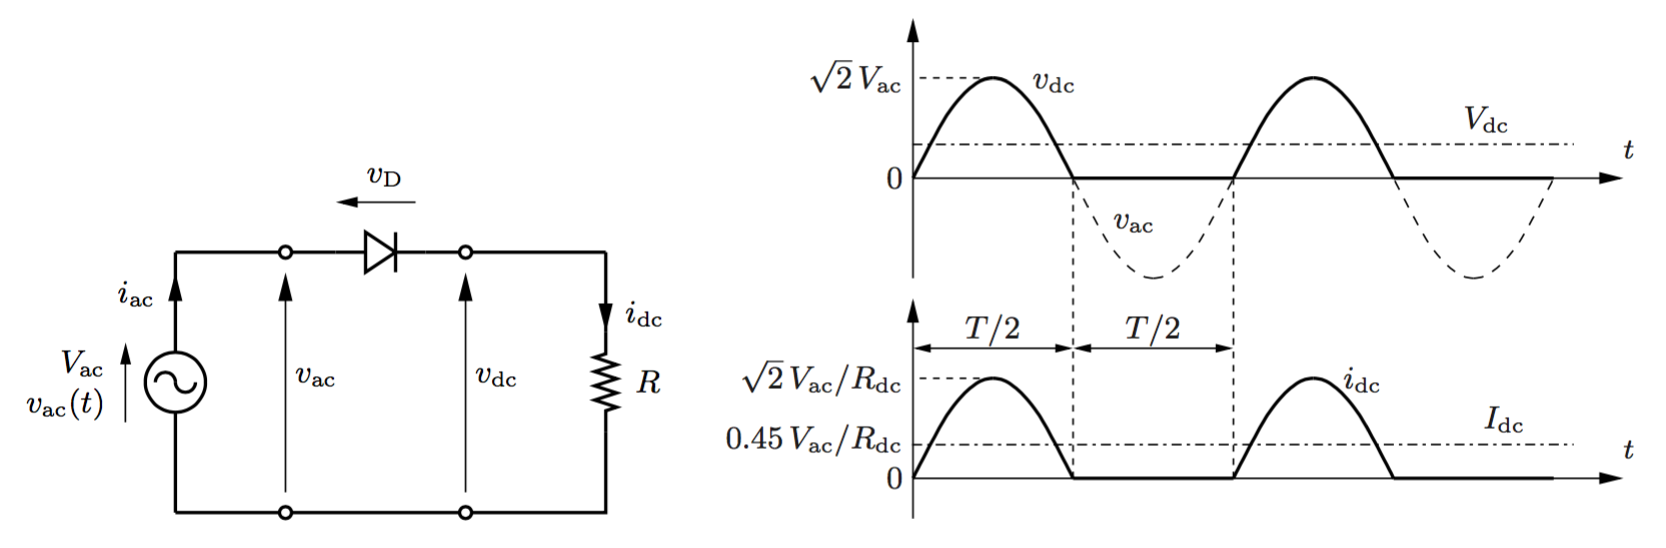
\includegraphics[scale=0.45]{ch2/3}
					\captionof{figure}{}
				\end{center}
				
				On obtient la valeur moyenne de la tension en intégrant sur une demi-période de conduction :
				\begin{equation}
					V_{dc} = \frac{1}{2\pi} \int _0^\pi \sqrt{2}V_{ac}\sin (\omega t) \, d\omega t = \underbrace{\frac{\sqrt{2}}{\pi}}_{0.450} V_{ac}.
					\label{eq:2.5}
				\end{equation}
				
				La tension redressée et le courant $i_{dc}=i_{ac}$ sont fortement ondulés, tous les harmoniques de fréquence $kf$ sont présents (pas de symétrie demi-onde). Le fait qu'un courant continu à moyenne non nul est tiré de la source pose un problème et provient d'un seul chemin $\Rightarrow$ \textbf{redresseur simple voie}. 
				
			\subsubsection{Avec charge ER}
				On a cette fois en plus une source de tension DC dans la charge et on peut voir le montage comme si on chargeait une batterie avec résistance interne. 
				
				\begin{center}
				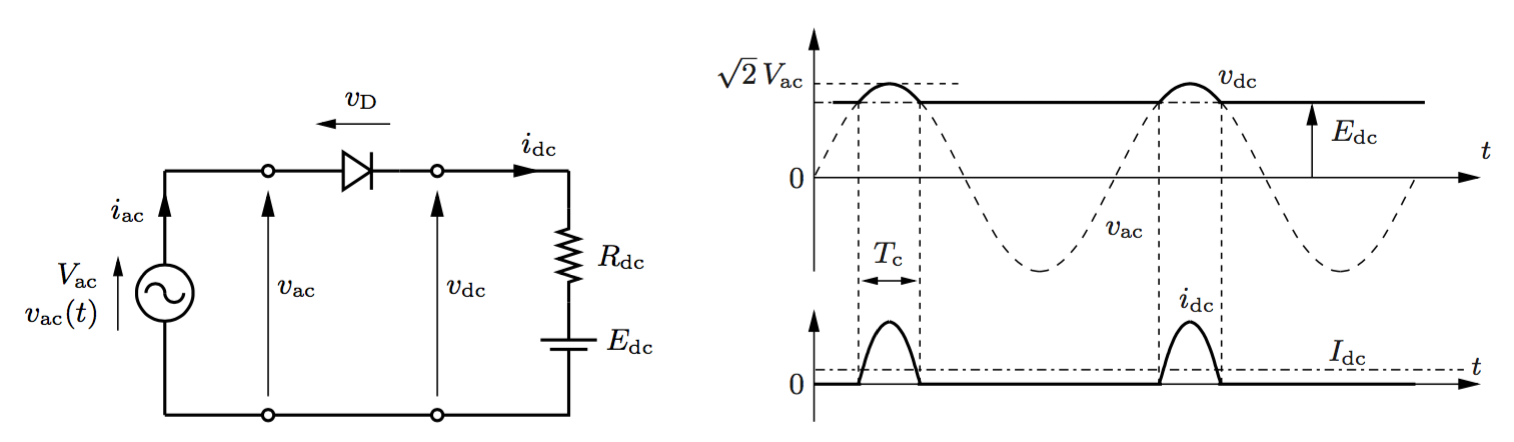
\includegraphics[scale=0.45]{ch2/4}
				\captionof{figure}{}
				\end{center}			 
				
				Dans le cas où la diode est passante, $v_{ac}(t) = v_{dc}(t) = E_{dc} + R_{dc}I_{dc}$, à la condition que $(v_{ac}-E_{dc})/R_{dc}>0$ donc que $v_{ac}>E_{dc}$. Dans le cas d'une diode bloquante, on a $v_{dc} = E_{dc}$. Les grandeurs DC déformées contiennent de nouveau tous les harmoniques de fréquence $kf$ et on a pour les intervalles de conduction de largeur $T_c$ ou $\theta _c = \omega T_c$ : 
				\begin{equation}
					E_{dc} = \hat{V}_{ac} \sin \left(\frac{\pi}{2} - \frac{\theta _c}{2}\right) = \hat{V}_{ac} \cos \frac{\theta _c}{2} \qquad \Rightarrow \qquad \theta _c = 2 \arccos \frac{E_{dc}}{\hat{V}_{ac}}
				\end{equation}
				où on remarque que les intervalles sont d'autant plus courts que $E_{dc}$ tend vers $\hat{V}_{ac}$. La tension $V_{dc}$ moyenne s'obtient en intégrant sur $\theta _c$ et les $2\pi - \theta _c$ restant : 
				\begin{equation}
				\begin{aligned}
					\frac{V_{dc}}{\hat{V}_{ac}} &= \frac{1}{2\pi\hat{V}_{ac}} \left[ \int _0 ^{2 \arccos \frac{E_{dc}}{\hat{V}_{ac}}} \hat{V}_{ac} \sin \omega t\,  d\omega t + \int _{2 \arccos \frac{E_{dc}}{\hat{V}_{ac}}} ^{2\pi} E_{dc} \, d\omega t \right]\\
								&= \frac{1}{\pi} \sqrt{1 - \left(\frac{E_{dc}}{\hat{V}_{ac}}\right)^2} + \left(1- \frac{1}{\pi} \arccos \frac{E_{dc}}{\hat{V}_{ac}} \right)
				\end{aligned}
				\end{equation}
				
	\subsection{Circuit avec une diode redresseuse et une diode de roue libre - empiétement}
		\begin{wrapfigure}[11]{l}{5.5cm}
		\vspace{-5mm}
		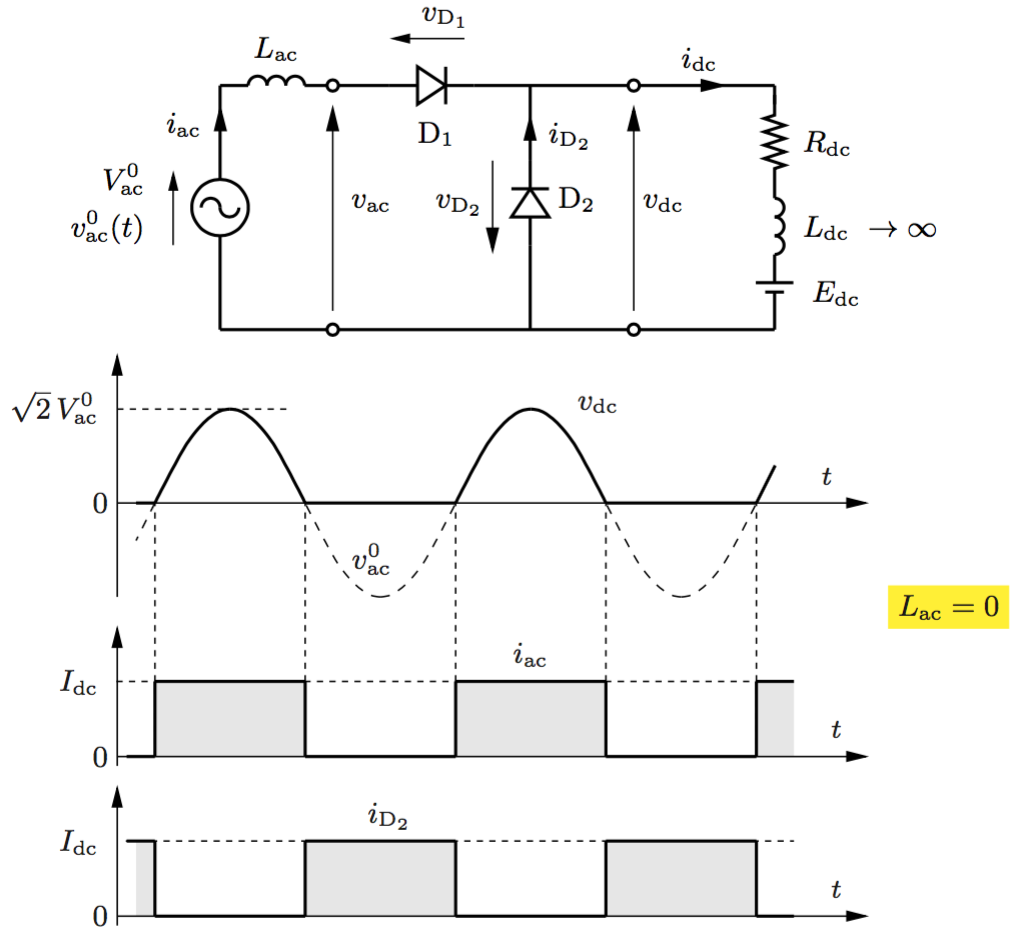
\includegraphics[scale=0.3]{ch2/5}
		\captionof{figure}{}
		\end{wrapfigure}
		Sur la figure ci-contre sont représentées deux diodes D1 et D2, la 1re laissant conduire la source de tension AC et la 2e dites de roue libre étant un chemin supplémentaire pour le courant dans la charge. La source AC est modélisée par son équivalent à vide $v_{ac}^0(t)$ et une inductance interne $L_{ac}$. Prenons d'abord le cas où $L_{dc} \rightarrow \infty$, lissant parfaitement le courant $i_{dc} = I_{dc}$. Il s'agit toujours d'un redresseur simple voie, car le courant n'est pas alternatif. \\\\\\
		
		\subsubsection{Avec source de tension AC idéale et charge infiniment inductive}
			Supposons d'abord que $L_{ac} = 0$, on a alors avec $L_{dc} = \infty$ : 
			\begin{equation}
				I_{dc} = i_{ac} + i_{D2}.
			\end{equation}
			
			On peut très bien faire l'expérience de la pensée qui conclut que le courant de la charge sera fourni par la source AC lors des alternances positives et circulera dans D2 lors des alternances négatives. La commutation entre les 2 diodes est instantanée. La valeur de tension moyenne se calcule comme \eqref{eq:2.5}. Lors des alternances négatives, la D2 étant passante, $-v_{D2} = v_{dc} = 0$. Toute la tension se retrouve alors sur D1.  
			
		\subsubsection{Avec source de tension AC non idéale et charge infiniment inductive}
			\begin{wrapfigure}[10]{l}{5.5cm}
			\vspace{-5mm}
			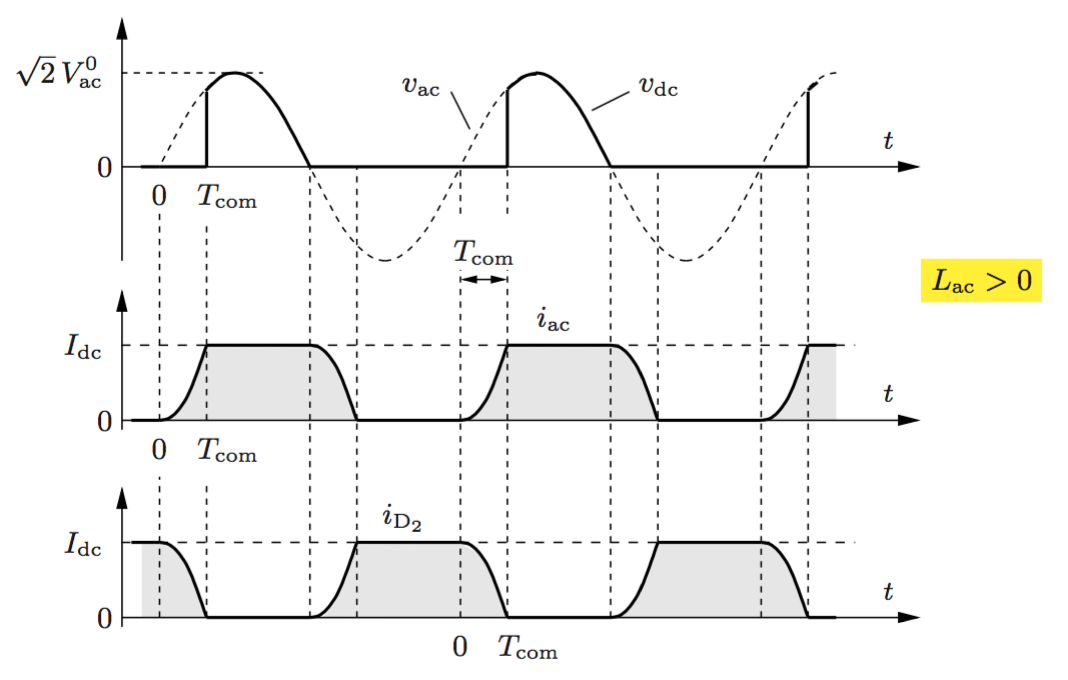
\includegraphics[scale=0.3]{ch2/6}
			\captionof{figure}{}
			\end{wrapfigure}
			Dans ce cas, $L_{ac}$ empêche les variations instantanées du courant lors des commutations. L'intervalle de temps est désigné par $T_{com}$, pendant lequel les 2 diodes conduisent en même temps, on parle d'\textbf{empiétement} ou de \textbf{recouvrement}. L'équation de la maille de gauche nous permet d'écrire avec les 2 diodes conductrices : 
			\begin{equation}
				v_{ac}^0 (t) = \sqrt{2} V_{ac}^0 \sin \omega t = Li_{ac}\frac{di_{ac}(t)}{dt}.
				\label{eq:2.9}
			\end{equation}
			On a comme précédemment $v_{dc}(t) = - v_{D2}(t) = 0$. Intéressons-nous dans un premier temps à la commutation de D2 vers D1 (0 à $T_{com}$). En intégrant \eqref{eq:2.9} comme suit : 
			\begin{equation}
			\begin{aligned}
				&\int _0 ^{\omega T_{com}} \sqrt{2} V_{ac}^0 \sin \omega t \, d\omega t = \int _0 ^{I_{dc}} \omega Li_{ac}\, di_{ac} \\
				\Leftrightarrow \quad &\sqrt{2} V_{ac}^0 (1- \cos \omega T_{com}) = \omega L_{ac} I_{dc}\\
				\Leftrightarrow \quad &\theta _{com} = \omega T_{com} = \arccos \left( 1 - \frac{\omega L_{ac}}{\sqrt{2} V_{ac}^0}I_{dc} \right)
				\end{aligned}
			\end{equation}			 
			On remarque ici que la durée de la commutation est d'autant plus grande que le courant et l'inductance sont grands. La commutation de $D_1$ vers $D_2$ se fait quoi qu'il en soit à $v_{dc} = 0$. Le retard sur la hausse de tension induit une baisse de la valeur moyenne de la tension de sortie désignée par $\Delta V_{com}$ : 			
			\begin{equation}
				\Delta V_{com} = \frac{1}{2\pi} \int _0 ^{\omega T_{com}} v_{ac}^0(t) \, d\omega t = \frac{1}{2\pi} \int _0 ^{\omega T_{com}} \omega L_{ac}\frac{di_{ac}}{dt} \, dt = \frac{\omega L_{ac}}{2\pi} I_{dc}.
 			\end{equation}
 			On voit que les mêmes conclusions sont valables pour la chute de tension moyenne.  
 
 		\subsubsection{Équivalent de Thévenin DC}
 			
			\begin{wrapfigure}[6]{r}{4cm}
			\vspace{-5mm}
			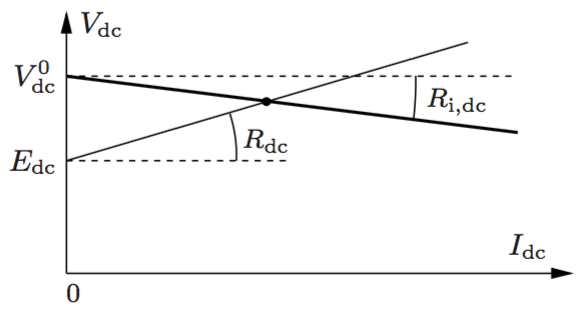
\includegraphics[scale=0.4]{ch2/7}
			\captionof{figure}{}
			\label{fig:2.6}
			\end{wrapfigure} 			
 			Si maintenant on prend en compte la chute de tension dans les diodes (identiques), on a : 
 			\begin{equation}
 				V_{dc} = \underbrace{0.45 V_{ac} - V_{D,on}}_{V_{dc}^0} - \underbrace{(R_{D,on}+\frac{\omega L_{ac}}{2\pi})}_{R_{i,dc}} I_{dc}
			\end{equation} 			 
			où on regroupe les termes sous un équivalent de Thévenin source de tension DC de la source AC et les 2 diodes, avec tension à vide $V_{dc}^0$ et résistance interne $R_{i,dc}$. Sur la \autoref{fig:2.6}, on peut voir le point de fonctionnement. Signalons qu'aucune perte Joule n'est associée à $R_{i,dc}$. 
			
		\subsubsection{Charge non infiniment inductive}
			Dans le cas d'une charge réelle avec $L_{dc}$ réel, on peut distinguer le cas d'une conduction ininterrompue donnant un courant $i_{dc}$ ondulé avec harmonique de fréquence $kf$ et toujours positif. On a aussi le cas d'une conduction interrompue avec $i_{dc} = 0$ durant des intervalles de temps (quand $i_{D2} >0$. Dans le cas \textbf{ininterrompu}, les équations pour $\theta _{com}$ et $\Delta V_{com}$ reste une bonne approximation, mais pour le cas \textbf{interrompu}, les équations sont fausses et la commutation de $D1$ vers $D2$ n'existe plus. 
			
\section{Ponts monophasé et triphasé - formules de base pour la tension redressée}
	\begin{wrapfigure}[7]{l}{8cm}
	\vspace{-5mm}
	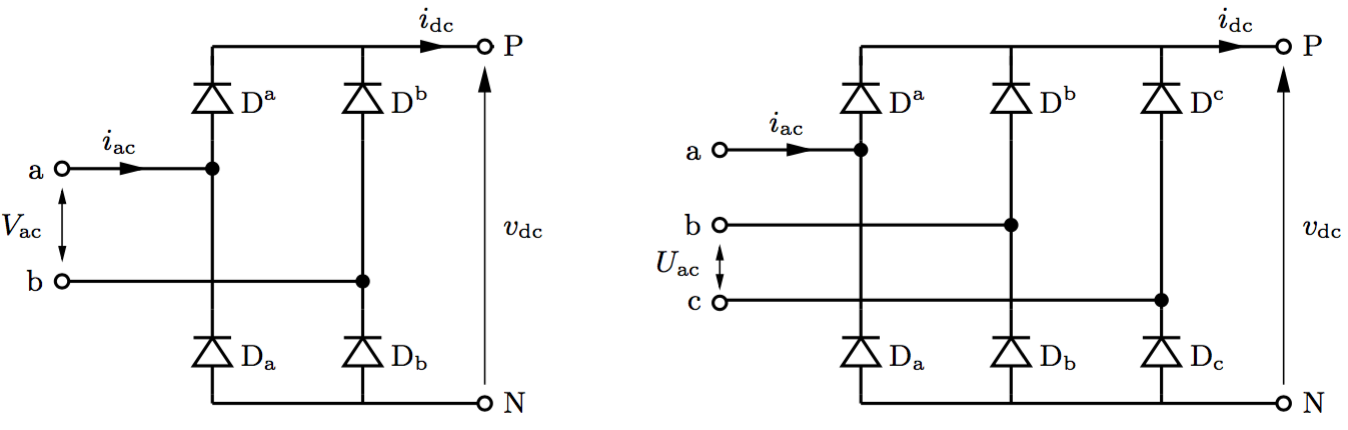
\includegraphics[scale=0.3]{ch2/8}
	\captionof{figure}{}
	\end{wrapfigure} 			
	La source de tension AC ) l'entrée est soit monophasée avec $V_{ac}$ pour tension efficace ou triphasée avec tension efficace $U_{ac}$ entre les lignes. La charge est connectée aux \textbf{bus positif P}  et \textbf{bus négatif N} avec tension de sortie instantanée $v_{PN}(t) \equiv v_{dc}(t)$. Puisque les alternances positives et négatives seront utilisées, on parle de \textbf{redresseur double voie}. Les bras des bornes d'entrée se raccordent aux points milieux. Le groupe de diodes supérieur constitue un sélecteur de potentiel maximum reliant le bus P à la borne d'entrée de potentiel max. Pareil pour le groupe inférieur qui constitue un sélecteur de potentiel minimum. Ainsi, $v_{PN} \equiv v_{dc}$ est le maximum des tensions entre lignes disponible à l'entrée. On a pour les deux cas : 
	\begin{equation}
	\begin{aligned}
		monophasé &: v_{dc}(t) = \max (v_{ac}, -v_{ac}) = |v_{ac}|,\\
		triphasé &: v_{dc}(t) = \max (u_{ab}, -u_{ab}, u_{bc}, -u_{bc}, u_{ca}, -u_{ca})
	\end{aligned}
	\end{equation}
	
	\begin{wrapfigure}[10]{r}{4cm}
	\vspace{-5mm}
	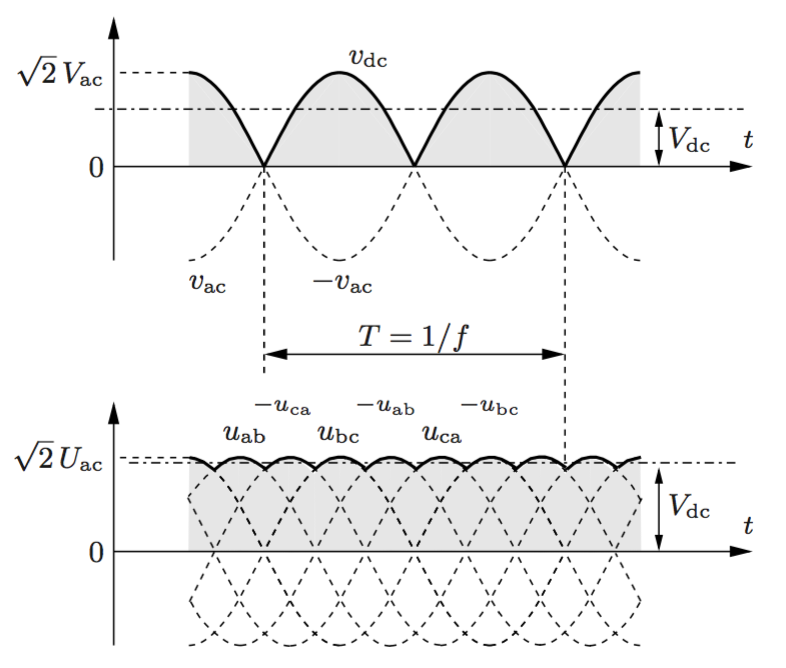
\includegraphics[scale=0.3]{ch2/9}
	\captionof{figure}{}
	\end{wrapfigure} 			
	Graphiquement, cela revient à considérer l'enveloppe supérieure des 2 ou 6 tensions comme illustré sur la figure ci-contre. On parle alors de redressement à 2 impulsions et redressement à 6 impulsions donnant des harmoniques de fréquences $2kf$ et $6kf$. La tension de sortie en triphasé est nettement moins ondulé, elle varie entre $\sqrt{3/4}Û_{ac} = 0.866 Û_{ac}$ à $Û_{ac}$. On a pour les valeurs moyennes :
	\begin{equation}
		\begin{aligned}
		monophasé &: V_{dc} = \frac{1}{\pi}\int _{-\frac{\pi}{2}} ^ {\frac{\pi}{2}} \sqrt{2} V_{ac} \cos \omega t \, d\omega t = \frac{2\sqrt{2}}{\pi} V_{ac},\\
		triphasé &: V_{dc} = \frac{3}{\pi}\int _{-\frac{\pi}{6}} ^ {\frac{\pi}{6}} \sqrt{2} U_{ac} \cos \omega t \, d\omega t = \frac{3\sqrt{2}}{\pi} U_{ac},
		\end{aligned}
		\label{eq:2.14}
	\end{equation}
	Les hypothèses sont les suivantes : 
	\begin{itemize}
		\item[•] La source de tension AC est supposée idéale alors que dans le réel on a une impédance. 
		\item[•] Diode conductrice à chaque instant, donc sans interruption. On peut avoir des intervalles durant lesquelles aucune diode ne conduit, où $v_{dc}$ ne dépendra que de la charge. 
		\item[•] Imperfection des diodes négligées. 
	\end{itemize}
	
\section{Ponts - fonctionnement avec charge inductive (conduction ininterrompue)}
	\subsection{Pont monophasé et charge infiniment inductive}
		\begin{wrapfigure}[8]{l}{5.5cm}
		\vspace{-5mm}
		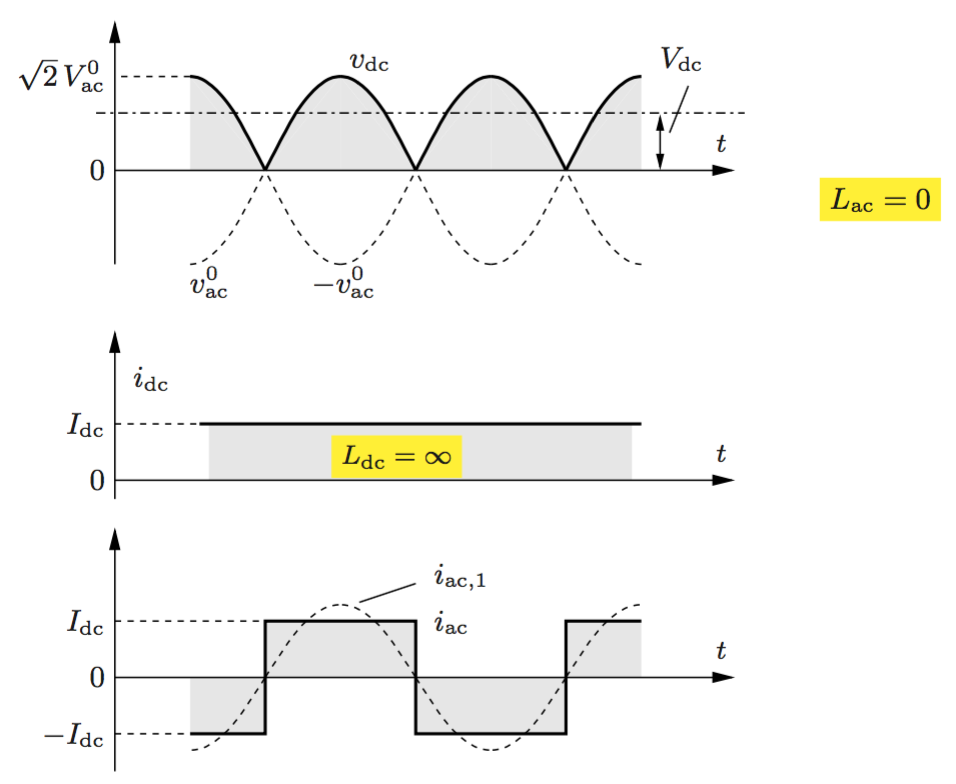
\includegraphics[scale=0.3]{ch2/10}
		\captionof{figure}{}
		\end{wrapfigure} 
		Source de tension AC idéale $L_{ac} = 0$ et charge RLE avec $L_{dc}\rightarrow \infty$. Lors des alternances positives de la tension d'entrée $v_{ac}^0$, les diodes $D^a$ et $D_b$ sont conductrices et durant les négatives $D^b$ et $D_a$. Le courant de sortie constant $i_{dc}$ donne un courant d'entré en onde carrée. C'est $L_{ac} = 0$ qui permet la discontinuité instantanée du courant. L'amplitude du fondamental du courant d'entrée vaut $I_{ac,1} = \frac{2\sqrt{2}}{\pi} I_{dc}$. Il est en phase avec $v_{ac}^0$ et donc le $DPF = \cos \varphi _1 \approx 1$, ce qui est le cas pour quasi tous les redresseurs à diodes. Le FP est par contre inférieur à l'unité vu la déformation du courant en onde carrée. On peut vérifier le bilan de puissance suivant à l'aide de l'équation \eqref{eq:2.14} : 
		\begin{equation}
			V_{ac}^0I_{ac,1} \cos \varphi _1 = V_{dc} I_{dc}.
		\end{equation}
		Lorsque $L_{dc} \neq \infty$, le courant n'est pas constant et oscille avec $I_{dc,min} \geq 0$. Lorsque $E_{dc}<V_{dc}$, le courant ne s'annule pas à condition que $L_{dc}$ soit suffisamment grand. Dans ce cas, on est dans l'ininterrompu et \eqref{eq:2.14} reste d'application. En prenant compte de la chute de tension dans les diodes, celle-ci devient en ininterrompu : 
		\begin{equation}
			V_{dc} = 0.9003V_{ac}^0 - 2 V_{D,on} - 2 R_{D,on} I_{dc}
		\end{equation}
		
	\subsection{Pont triphasé et charge infiniment inductive}
		\begin{wrapfigure}[12]{l}{5.6cm}
		\vspace{-5mm}
		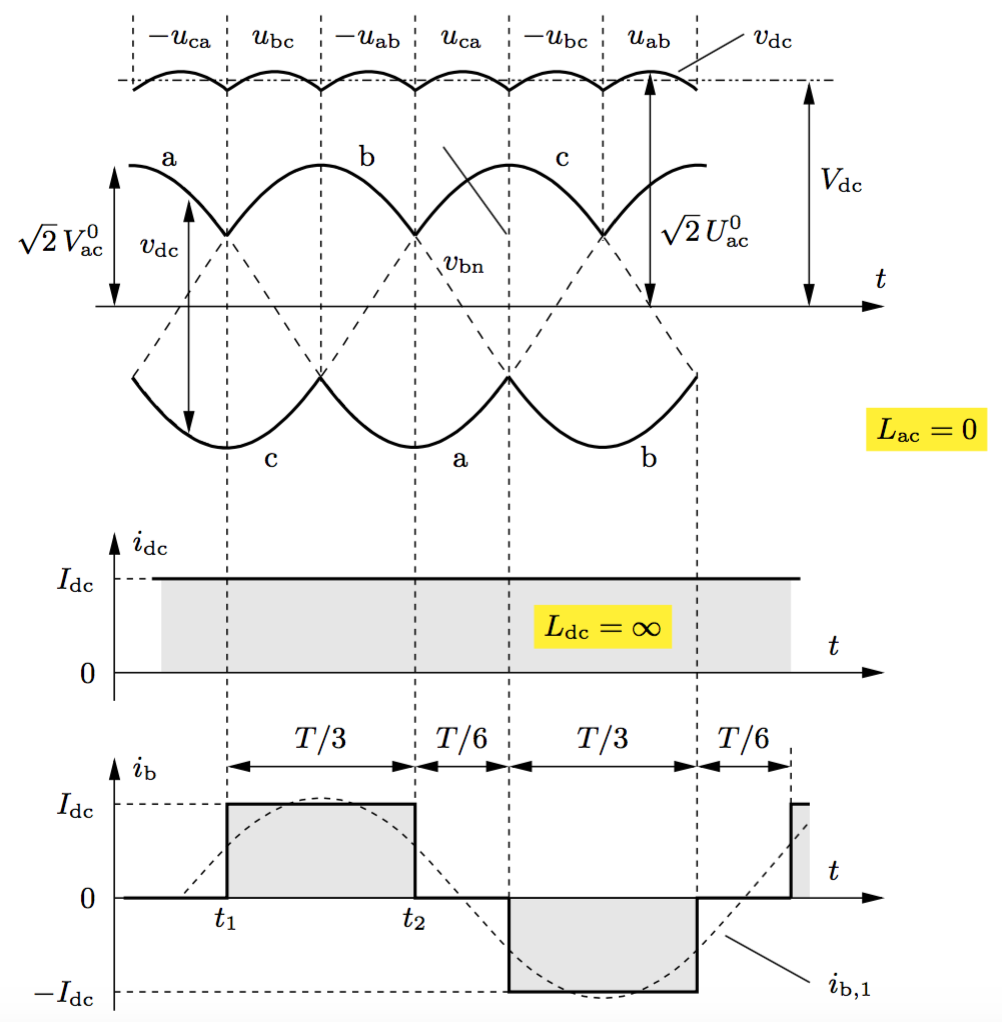
\includegraphics[scale=0.3]{ch2/11}
		\captionof{figure}{}
		\end{wrapfigure} 
		La source de tension idéale est représentée par son équivalent en étoile. On suppose $L_{dc} = \infty$ et les 3  phases contribuent de façon symétrique au courant continu et constant. Durant une période fondamentale, chaque phase conduit durant 2 fois 120\degres et ne conduit pas durant 2 fois 60\degres . Comme précédemment, les 3 courants ont une forme d'onde carrée triphasée. On a à nouveau les  fondamentales de courant en phase avec les tensions des phases correpondntes et $\phi _1 = 0 \Rightarrow \cos \phi _1 = 1$. La valeur efficace de la composante fondamentale du courant vaut $I_{ac,1} = \frac{\sqrt{6}}{\pi}I_{dc}$. Ainsi le bilan de puissance :

		\begin{equation}
			\sqrt{2}V_{ac}I_{ac,1} \cos \phi _1= V_{dc}I_{dc}. 
		\end{equation}
		
		Dans le cas \textbf{ininterrompu}, \eqref{eq:2.14} reste valable en y ajoutant les pertes des 2 diodes conductrices. 
		
	\subsection{Commutation entre diodes en présence d'inductance AC}
		On peut, en plus de l'inductance de la source, avoir une inductance de lissage ou un filtre LC en amont des diodes. La commutation ne peut alors se faire instantanément. \\
		
	\begin{wrapfigure}[8]{r}{5cm}
		\vspace{-5mm}
		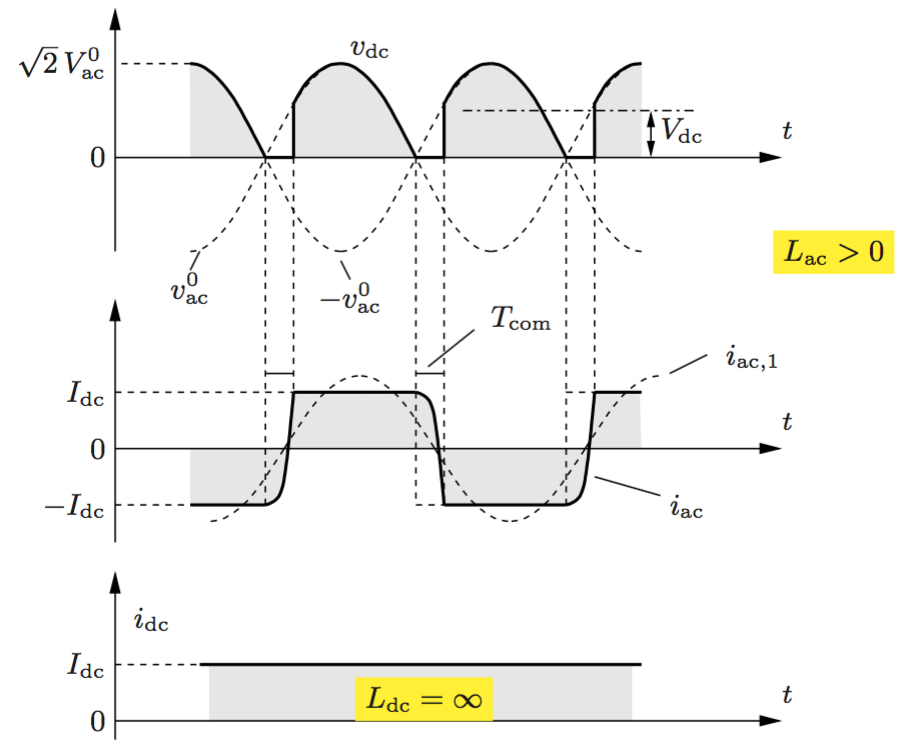
\includegraphics[scale=0.3]{ch2/12}
		\captionof{figure}{}
		\end{wrapfigure} 
		Regardons d'abord le cas monophasé avec inductance après source $L_{ac} \neq 0$. La figure ci-contre nous montre les intervalles de commutation $T_{com}$. On peut montrer que dans le cas d'une charge infiniment inductive, la tension de sortie sera la moyenne des deux présentes lors de la commutation, donc nulle. On a alors pour la durée de commutation : 
		\begin{equation}
			\omega T_{com} = \arccos \left( 1-\frac{2\omega L_{ac}}{\sqrt{2}V_{ac}} I_{dc}\right). 
		\end{equation}
		
		On trouve alors pour la diminution de la moyenne : 
		\begin{equation}
			\Delta V_{dc} = \frac{2\omega L_{ac}}{\pi}I_{dc}. 
		\end{equation}
		
		\begin{wrapfigure}[5]{l}{4cm}
		\vspace{-5mm}
		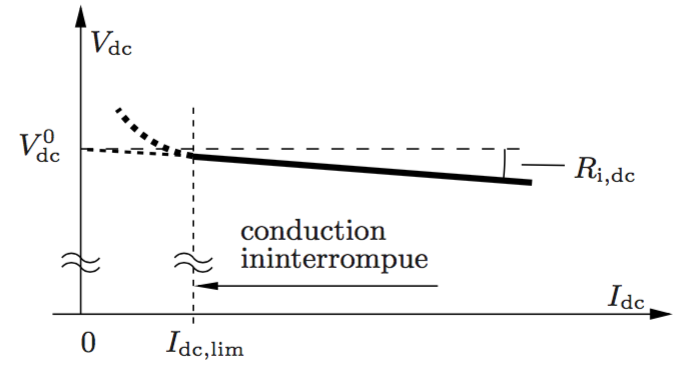
\includegraphics[scale=0.3]{ch2/13}
		\captionof{figure}{}
		\end{wrapfigure} 
		On peut alors exprimer la tension moyenne avec les chutes aux diodes et $\Delta V_{dc}$ puis regrouper en source de tension continue avec sa résistance interne (Thévenin) : 
		\begin{equation}
			V_{dc} = \underbrace{0.9003 V_{ac}^0 - 2V_{D,on}}_{V_{dc}^0} - \underbrace{\left( 2 R_{D,on} + \frac{2\omega L_{ac}}{\pi} \right)}_{R_{i,dc}} I_{dc}
		\end{equation}		 
		Valable uniquement dans le cas d'une conduction ininterrompue, caractérisée par une valeur seuil $I_{dc,lim}$. Comme effet secondaire du recouvrement, la composante fondamentale du courant est déphasée par rapport à la tension à vide $v_{ac}^0$ avec $\phi _1 >0$ et $DF = \cos \phi _1 < 1$. \\
		
		Dans le cas triphasé, les équations obtenues (livre de référence) sont : 
		\begin{equation}
			\omega T_{com} = \arccos \left( 1-\frac{2\omega L_{ac}}{\sqrt{2}U_{ac}^0} I_{dc}\right) \qquad \Delta V_{com} = \frac{3\omega L_{ac}}{\pi} I_{dc}.
		\end{equation}
		
\section{Ponts - fonctionnement avec lissage de la tension redressée}
	On branche une capacité C en parallèle sur la charge pour lisser la tension. La déformation de $v_{dc}(t)$ sera d'autant plus faible que C sera grand. Le cas d'une capacité infinie donne lieu à une tension parfaitement lisse $V_{dc}$ (nécessité d'une énergie et un temps de charge infini). La charge sera pour l'instant considérée comme une résistance $R_{dc}$. La tension $v_{dc}(t) = v_C(t)$ est liée aux courants :
	\begin{equation}
		C\frac{dv}{dt} = i_C = i_{dc} - i_{dc,R}
		\label{eq:2.22}
	\end{equation}
	où $i_{dc}$ et $i_{dc,R} > 0$. En régime établi, $I_C = 0$. On a alors $I_{dc} = I_{dc,R}$ et est d'autant plus grand que la résistance est petite (charge grande). En absence de charge $R_{dc}=\infty$, aucune conduction dans le pont. 
	
	\subsection{Ponts à diodes monophasés}
		\begin{wrapfigure}[7]{r}{7.5cm}
		\vspace{-5mm}
		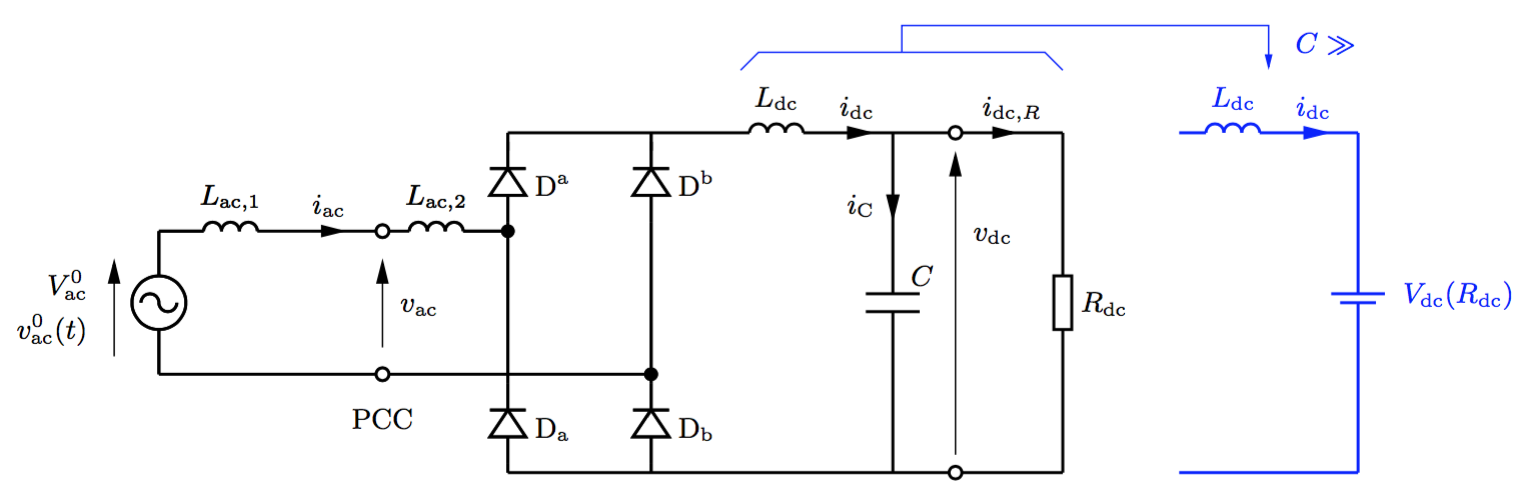
\includegraphics[scale=0.3]{ch2/14}
		\captionof{figure}{}
		\end{wrapfigure} 
		Le circuit ci-contre possède 3 impédances, une liée à la source $L_{ac,1}$, bobine de lissage à l'entrée $L_{ac,2}$ et une deuxième bobine de lissage en amont du condensateur $L_{dc}$. On néglige les différentes résistances internes. D'autres charges peuvent être raccordées à la même source de tension AC via le PCC, où la tension est :
		
		\begin{equation}
			v_{ac}(t) = v_{ac}^0(t) - L_{ac,1}\frac{di_{ac}}{dt}.
		\end{equation}
		
		Si on suppose $v_{ac}^0$ parfaitement sinusoïdale (pas d'harmonique), la seule déformation est due à celle du courant $i_{ac}$. Explicitons les harmoniques de rang $k>1$ de $v_{ac}^0(t)$ et $i_{ac}(t)$ et leurs valeurs efficaces :
		
		\begin{equation}
			v_{ac,k}(t) = -L_{ac,1}\frac{di_{ac,k}}{dt} \qquad \Rightarrow  V_{ac,k} = k\omega L_{ac,1} I_{ac,k}.
		\end{equation}
		Il importe donc de limiter la déformation du courant pour limiter celle de la tension. Grâce au condensateur, la tension de sortie est peu ondulée et on peut modéliser l'ensemble condensateur-résistance comme une source de tension DC idéal, mais dont $V_{dc}=cst$ dépend de la valeur de $R$. 
		
		\subsubsection{Conduction interrompue}
			\begin{wrapfigure}[7]{l}{6cm}
			\vspace{-5mm}
			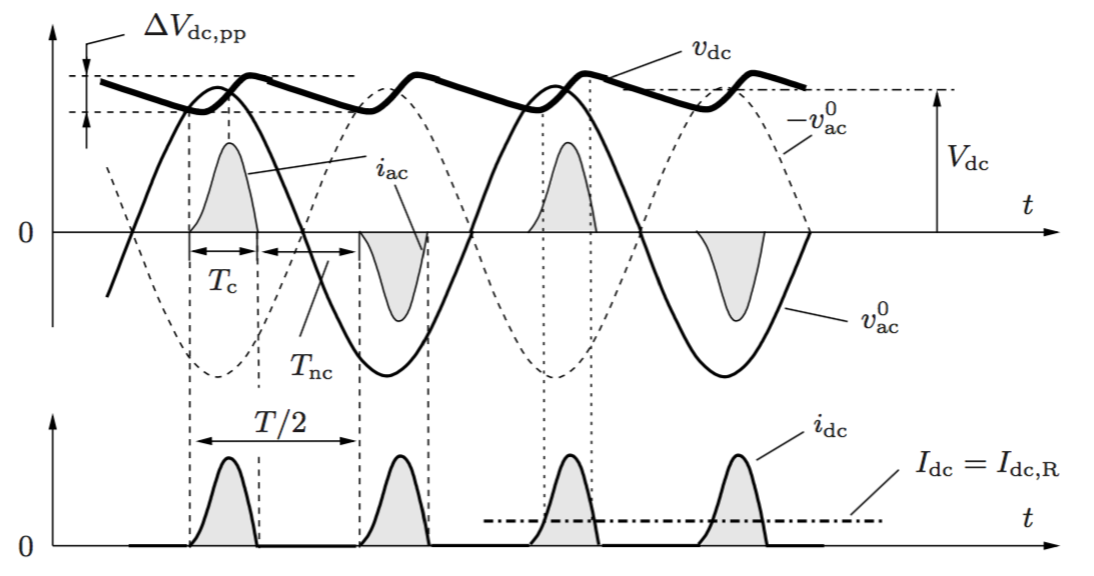
\includegraphics[scale=0.3]{ch2/15}
			\captionof{figure}{}
			\end{wrapfigure} 
			Sur la figure ci-contre on peut voir l'ondulation de la tension de sortie. Comme il existe des intervalles $T_{nc}$	durant lesquelles $i_{ac} = 0$, la conduction est interrompue. Ces intervalles sont délimités par des impulsions de courant positives et négatives, chacune de durée $T_{c}$, avec :
			\begin{equation}
				T_{nc} + T_c = \frac{T}{2}.
			\end{equation}
			
			La conduction se fait par paire de diodes, sans recouvrement (4 diodes en même temps). Le courant redressé $i_{dc}$ n'est rien d'autre que $|i_{ac}|$ et possède donc 2 impulsions positives par période fondamentale. Le courant $i_{ac} \neq 0$ n'apparaît que lorsque $|v_{ac}^0(t)| \geq v_{dc}(t)$. Grâce à l'inductance totale $L_{ac} + L_{dc}$, $i_{ac}$ croît graduellement pour atteindre son max lorsque $|v_{ac}^0| = v_{dc}$. La conduction perdure tant que les inductances restituent l'énergie accumulée. Pendant les intervalles de conduction $T_c$, l'équadiff pour la montée et la descente de $i_{dc}$ est :
			\begin{equation}
				(L_{ac}+L_{dc})\frac{d_{i_{dc}}}{dt} = |v_{ac}(t)|-v_{dc}(t).
			\end{equation}
			
			\textbf{Tension de sortie} \qquad Dans le cas réel où $C$ est fini, $v_{dc}(t)$ est en \textit{dents de scie}. L'ondulation est d'autant plus faible que C est grand. Durant $T_{nc}$ où $i_{dc} =i_{ac} =0$, aucun courant n'est fournit au condensateur, mais ce dernier alimente la charge en se déchargeant faiblement. Si la constante de temps $\tau = R_{dc}C$ est grande devant $T/2$, les flancs descendant des dents-de-scie sont pratiquement droits et de pente $-V_{dc}/\tau$ : 
			\begin{equation}
				C\frac{v_{dc}(t)}{dt} = -i_{dc,R}(t) = \frac{v_{dc}(t)}{R} \qquad \Rightarrow \qquad \frac{dv_{dc}}{dt} \approx - \frac{V_{dc}}{R_{dc}C} \qquad (i_{dc} = 0).
			\end{equation}
			
			Durant un intervalle de conduction $T_c$, $v_{dc} = v_c$ atteint une valeur extrémale lorsque $i_{dc} = i_{dc,R}$ selon \eqref{eq:2.22}. En particulier, on a un minimum au début et un maximum à la fin de $T_c$. L'ondulation crête à crête de $v_{dc}(t)$ est approché comme suit :
			\begin{equation}
				\Delta V_{dc,pp} \approx \frac{T_{nc}}{R_{dc}C}V_{dc},
			\end{equation}
			dont une limite supérieure s'obtient avec $T_{nc} = T/2$.
			\\
			
			\textbf{Courant de sortie} \qquad Puisque $v_{dc}$ est peu ondulé, il en est de même pour $i_{dc} = v_{dc}/R_{dc}$. Le courant dans le condensateur $i_c = i_{dc}-i_{dc,R}$ est la différence entre $i_{dc}$ en impulsions $\pm$ étroite et $i_{dc,R}$ quasi constante. Pour rappel, $i_c$ est un courant AC de valeur nulle (régime). 
			\\
			
			\textbf{Caractéristique tension/courant de sortie adimensionnelle} \qquad On s'intéresse à la caractéristique de sortie globale, la tension de sortie moyenne $V_{dc}$ versus $I_{dc}$ c'est-à-dire la résistance de charge $R_{dc}=V_{dc}/I_{dc}$, en supposant une capacité suffisamment grande que pour négliger son effet sur la caractéristique. Les paramètres restants sont 

			\begin{wrapfigure}[6]{r}{6cm}
			\vspace{-5mm}
			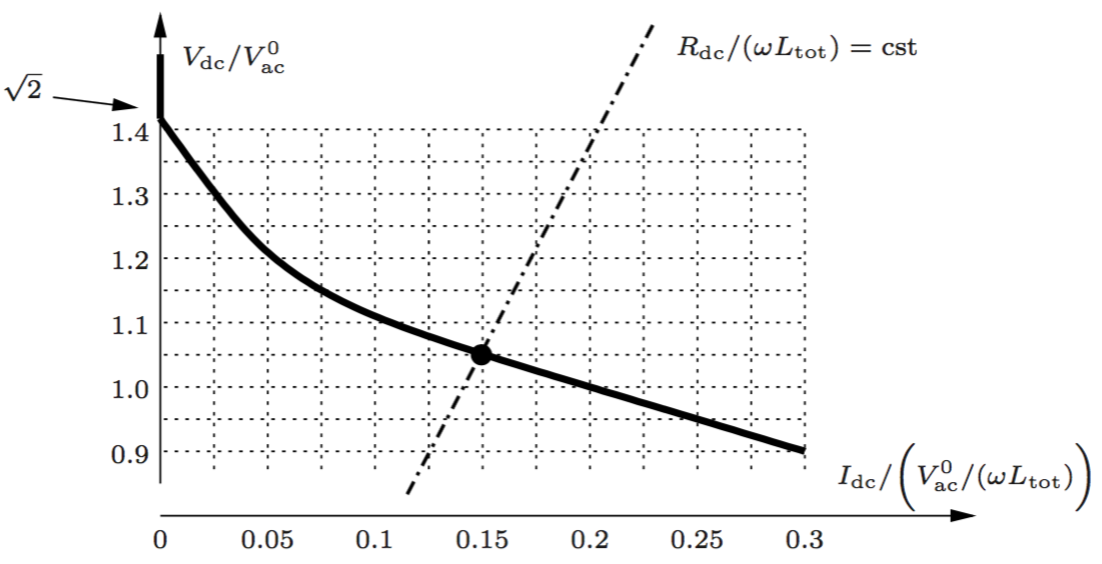
\includegraphics[scale=0.3]{ch2/16}
			\captionof{figure}{}
			\end{wrapfigure} 
			alors $V_{ac}^0, \omega$ et $L_{tot}$ (pour le cas interrompu). En rendant adimensionnels $V_{dc}$ et $I_{dc}$ en divisant par $V_{ref} = V_{ac}^0$ et $I_{ref} = V_{ac}^0/(\omega L_{tot})$, on représente la caractéristique de sortie par la seule courbe de la figure ci-contre. Elle est valable quelle que soit les valeurs de $V_{ac}^0, \omega$ et $L_{tot}$ tant que C est grand. On voit que $V_{dc}$ est d'autant plus proche 
			\newpage 
			de $\sqrt{2}V_{ac}^0$ que la charge est diminuée ($R_{dc}$ croissant, $I_{dc}$ décroissant). En absence de charge ($R_{dc} = \infty$, $I_{dc} = 0$), le condensateur reste chargé à une tension d'au moins $\sqrt{2}V_{ac}^0$ et aucun courant ne circule dans le pont à diode. \\
			Lorsqu'on augmente la charge ($R_{dc}$ décroissant), on descend sur la courbe, $V_{dc}$ diminue et $I_{dc}$ augmente. Cela va de pair avec l'augmentation de la durée $T_c$. On atteint finalement la limite entre les conductions interrompue et ininterrompue, où l'on a $T_c = T/2$ et où les impulsions de courant se rejoignent. Par simulation numérique, cette limite se trouve à $I_{dc} \approx 0.3 V_{ac}^0/(\omega L_{tot})$, correspondant au point {0.3, 0.9} de la courbe. Le THD de $i_{ac}(t)$ tend à être assez grand lorsque la charge est légère. En contrepartie, le déphasage de la composante fondamentale de $i_{ac}(t)$ avec $v_{ac}(t)$ est faible, donnant un DPF $\cos \varphi _1 \approx 1$. 
			
		\subsubsection{Conduction ininterrompue}
			\begin{wrapfigure}[8]{l}{6cm}
			\vspace{-5mm}
			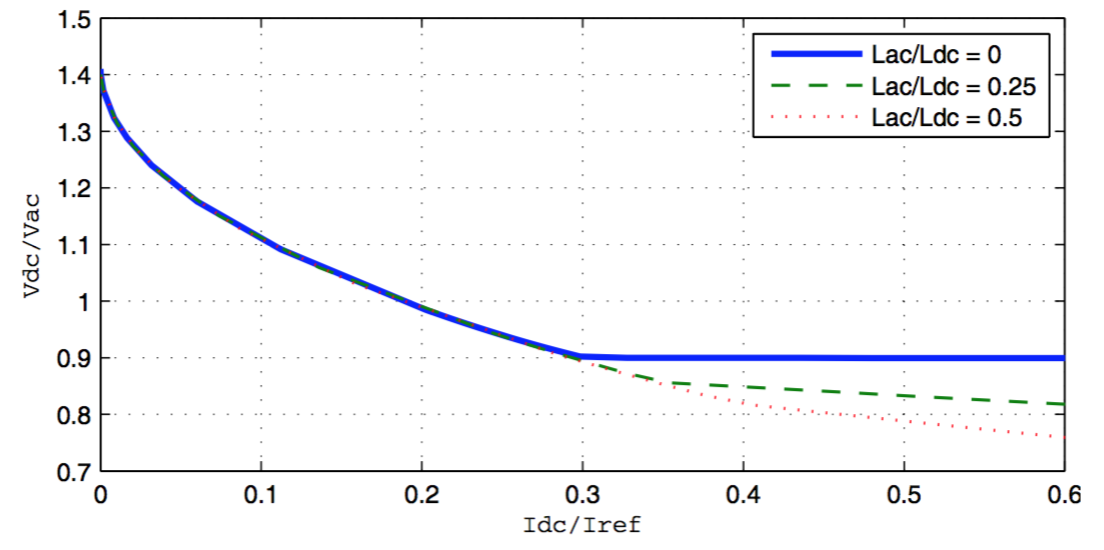
\includegraphics[scale=0.3]{ch2/17}
			\captionof{figure}{}
			\end{wrapfigure} 
			Dans ce cas, quand $I_{dc}/I_{ref}>0.3$ l'étude menée redevient pertinente. La tension $v_{dc}$ essentiellement constante grâce au condensateur correspond à $E_{dc}$ de la charge. $L_{dc}$ correspond à l'inductance de la charge et n'a que peu d'influence sur la tension. Par contre $L_{ac}$ est responsable de l'empiétement qui annule la tension de sortie. Par 3 séries de simulations avec des valeurs différentes de $L_{ac}$ et $L_{dc}$ tout en ayant la même $L_{tot}$, avec une large plage pour $R_{dc}$ et une grande capacité, on obtient les 3 courbes ci-contre. Dans la plage $0<I_{dc}/I_{ref}<0.3$, la conduction est ininterrompue et les courbes sont confondues, ce qui montre que c'est $L_{tot}$ qui est pertinente et pas celles prises séparément. Pour des courants adimensionnels plus importants, la tension adimensionnelle diminue linéairement avec le courant en raison de l'empiétement qui est influencé uniquement par $L_{ac}$.
			
	\subsection{Ponts à diodes triphasés}
	
		\begin{center}
		\begin{minipage}{0.45\textwidth}
			\begin{flushleft}
			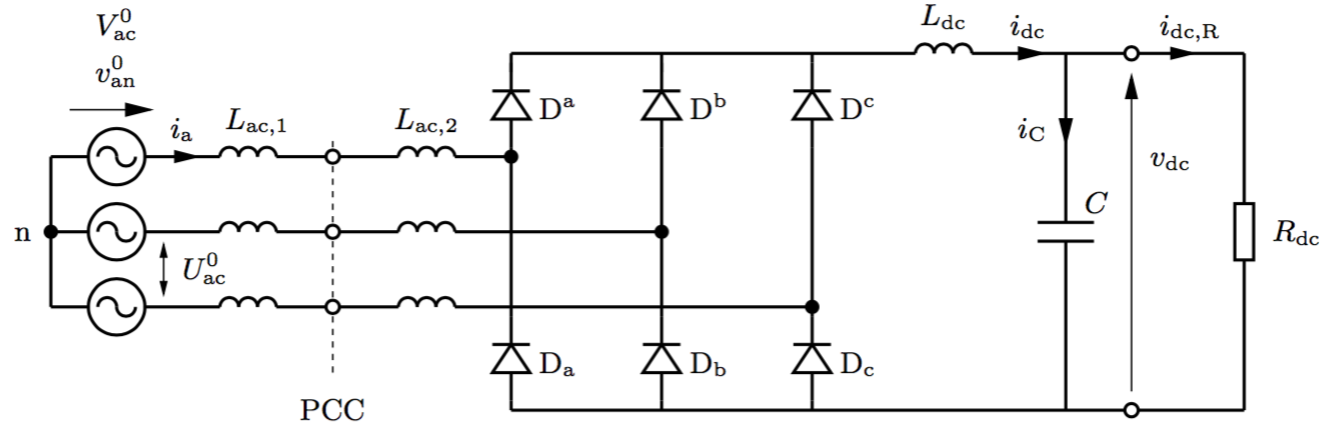
\includegraphics[scale=0.4]{ch2/18}
			\captionof{figure}{}
			\end{flushleft}
		\end{minipage}			
		\begin{minipage}{0.45\textwidth}
			\begin{flushright}
			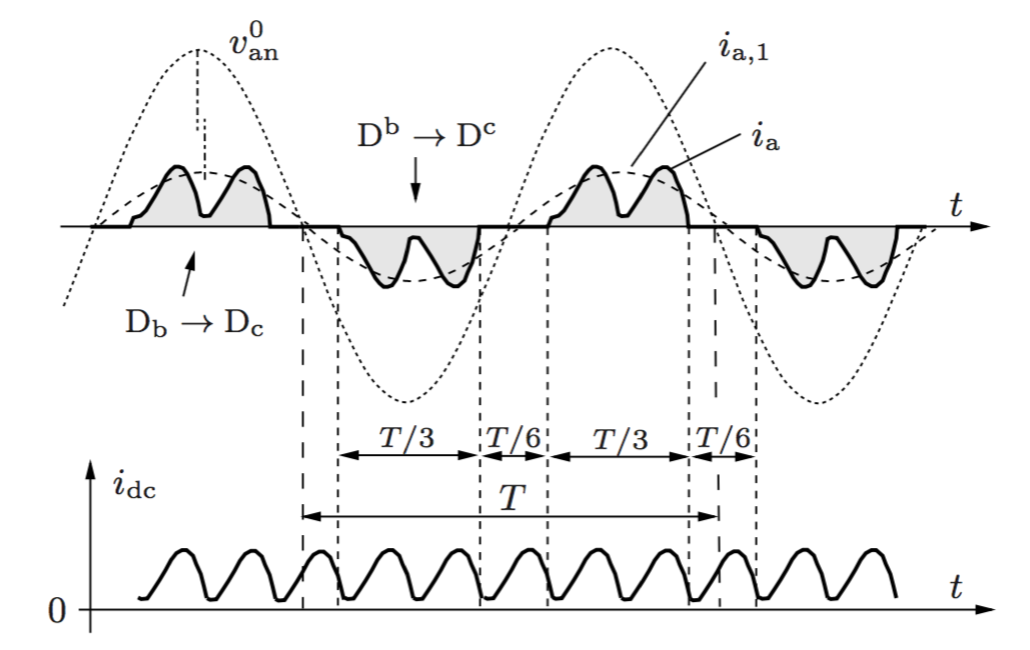
\includegraphics[scale=0.4]{ch2/19}
			\captionof{figure}{}
			\end{flushright}
		\end{minipage}			
		\end{center}
		
		Voici le montage équivalent en triphasé, chaque ligne d'entrée comprennent les inductances $L_{ac,1}$ et $L_{ac,2}$ alors qu'un seul $L_{dc}$ se situe en amont du condensateur. L'allure typique du courant AC tiré de la source est également représentée, dans le cas de conduction ininterrompue où le courant de phase comprend 2 intervalles de conduction de 120\degres . Le creux par intervalle de conduction d'une phase correspond à la commutation entre les deux autres phases comme indiqué sur la figure ci-dessus.\\
		
		\textbf{Conduction interrompue}\qquad Lorsque la charge est diminuée ($R_{dc}$ augmentée) et que la conduction devient interrompue le courant AC comprend 2 impulsions positives bien séparée et pareille pour les impulsions négatives par période d'alimentation AC. On a alors $i_{dc} = |i_{ac}|$ et lors des intervalles de conduction le courant circule dans $L_{dc}$, 2 des six diodes, deux des 3 $L_{ac}$ d'entrée. \\
		
		\begin{wrapfigure}[8]{l}{6cm}
		\vspace{-5mm}
		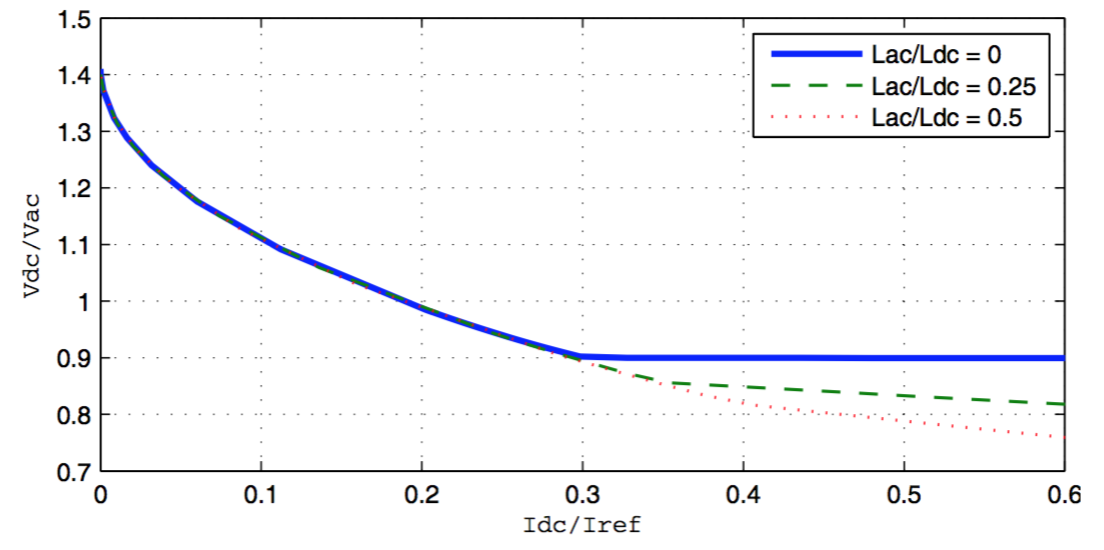
\includegraphics[scale=0.3]{ch2/17}
		\captionof{figure}{}
		\end{wrapfigure} 
		\textbf{Caractéristique tension/courant de sortie adimensionnelle}\qquad 		 On définit cette fois comme valeurs de référence $V_{ref} = U_{ac}^0$ et $I_{ref} = I_{ac}/(\omega L_{tot})$. Il convient cette fois de définir $L_{tot} = L_{dc}+ 2L_{ac}$. La même simulation que le cas monophasé est appliquée et les courbes obtenues sont reportées sur le graphe ci-contre. On y observe que la limite entre conduction interrompue et ininterrompue et située vers $I_{dc}/I_{ref} = 0.013$ et que le rapport 1.35 entre $V_{dc}$ et $U_{ac}^0$ de la conduction ininterrompue se confirme.
